\documentclass[a4paper,10.5pt]{report}
\usepackage[T1]{fontenc}
\usepackage[utf8]{inputenc}
\usepackage[french]{babel}
\usepackage{empheq}
\usepackage{mathtools, bm}
\usepackage{amssymb, bm}
\usepackage{graphicx}
\usepackage{caption}
\usepackage{subcaption}
\usepackage{hyperref}
\usepackage{amsfonts}

\title{\textbf{\Huge  Université Paris Sud}\\ PROJET IGSD 2019}
\author{Coquisart Jérôme}
\date{15 janvier 2020}


\begin{document}
    \maketitle
    \newpage
    \tableofcontents
    \newpage

    \chapter*{Introduction}
    \addcontentsline{toc}{chapter}{Introduction}

    \begin{figure}[h!]
        \centering
        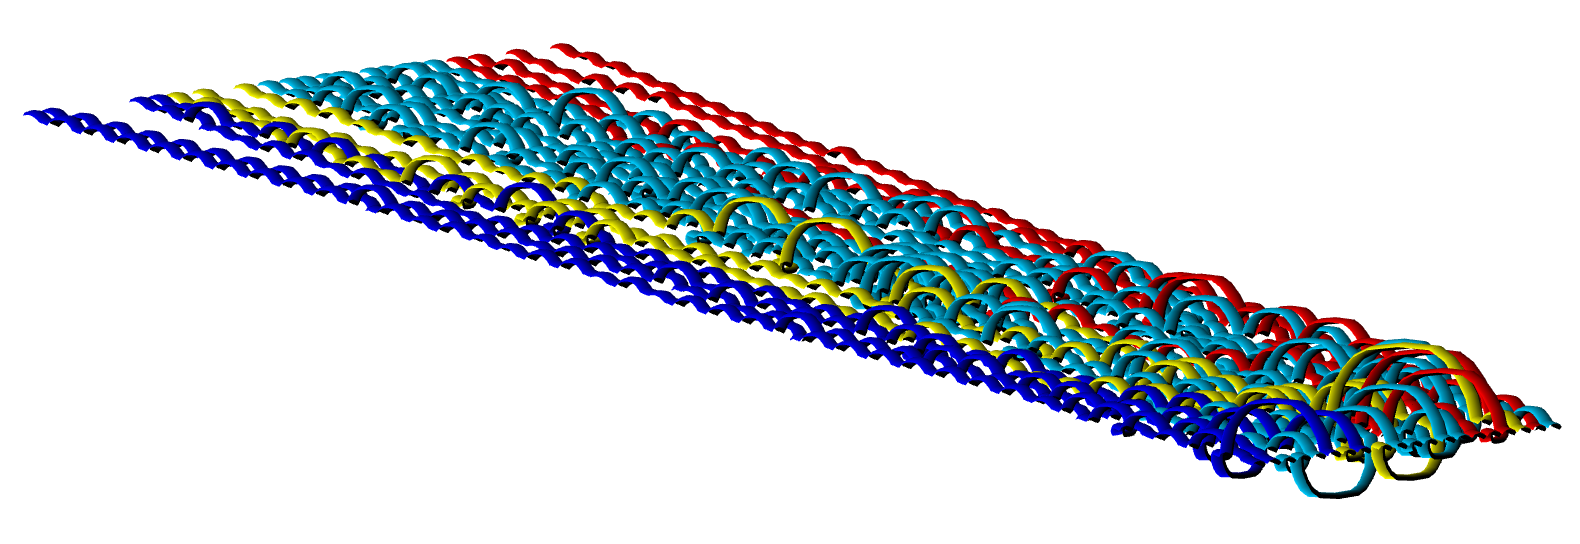
\includegraphics[height=4cm]{../main2.png}
        \caption{Vue globale en 3D}
    \end{figure}
    L'objectif de ce projet est de se familiariser avec le moteur graphique \textbf{OpenGL} en C++.
    Nous avons réalisé des gapchart en trois dimension suivant le classement des équipes du Premier League, le championnat de foot du Royaume-Unis.
    Ce rapport est organisé selon les questions du \href{http://vernier.frederic.free.fr/Teaching/IGSD/Projet2019-3gGapchart.pdf}{sujet du projet}.
    Il est possible de reproduire chaque figure en déplacant la caméra (voir \ref{sec:caméra-2d} et \ref{sec:caméra-3d}).

    \begin{figure}[h!]
        \centering
        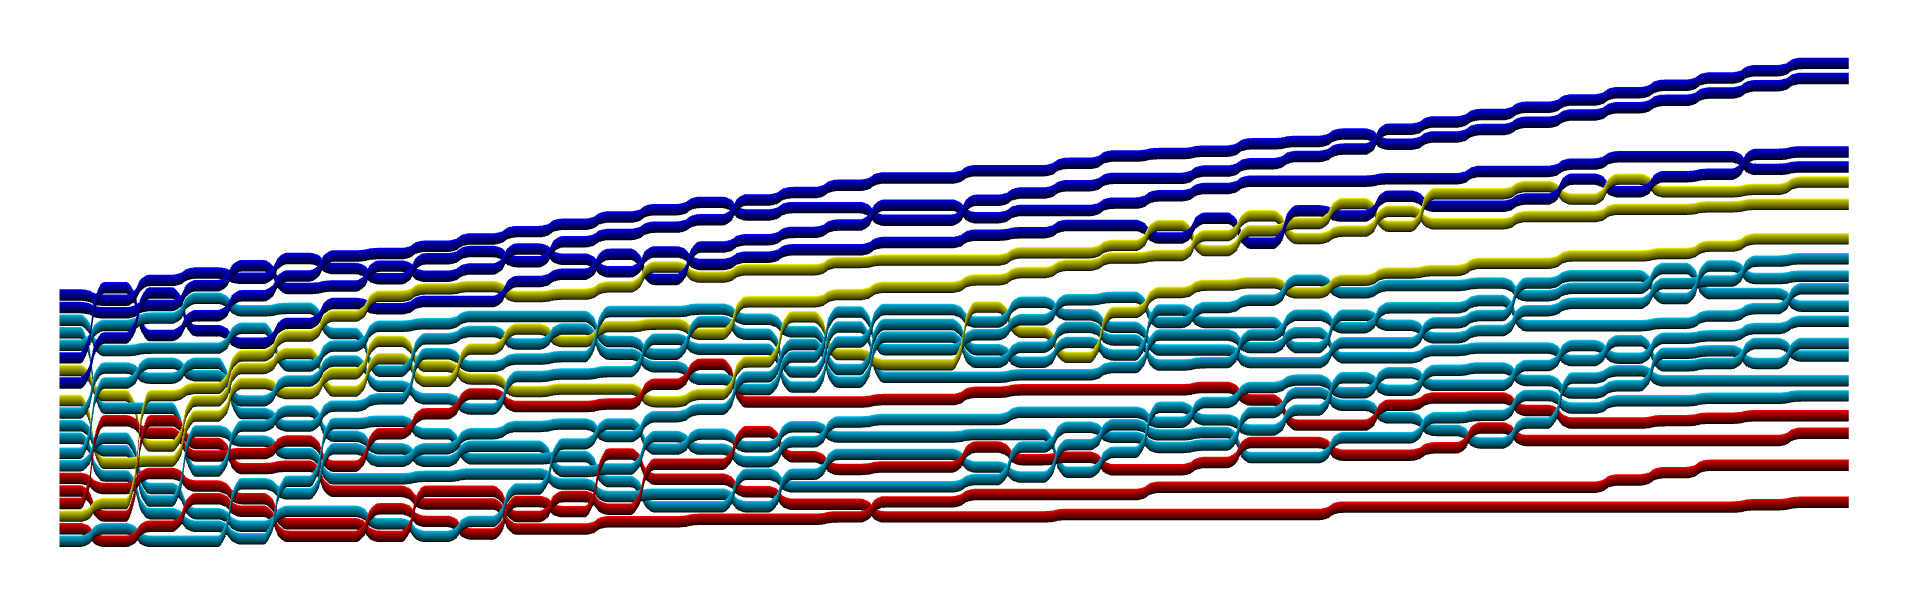
\includegraphics[width=13cm, height=6cm]{../main.png}
        \caption{Vue globale en 2D}
    \end{figure}

    \chapter{Données}\label{ch:données}
    À partir du fichier \textit{.csv} et après avoir implémenté la fonction \textit{LoadData}, on récupère le classement et le nombre de point des 20 équipes.
    Pour aller un peu plus loin, nous avons créé un tableau qui contient l'historique des adversaires rencontrés.
    Cela sera utile pour les arcs de cerlce (voir~\ref{arc}).
    \chapter{Modèle 3D}\label{ch:modèle-3d}
    \section{Création des courbes et "S"}\label{sec:création-des-courbes-et-"s"}
    Nous avons créé un VBO par courbe qui décrit les sommets des triangles permettant de dessiner chaque courbe.
    Une fonction calculant les ordonnées de chaque point a été très utile pour manipuler les courbes.
    Puis on dessine les demi-cylindres autour de chaque ordonnée avec $y\mapsto \cos(y)$ et $z\mapsto\sin(z)$.

    \begin{figure}[h!]
        \begin{subfigure}[t]{.6\textwidth}
            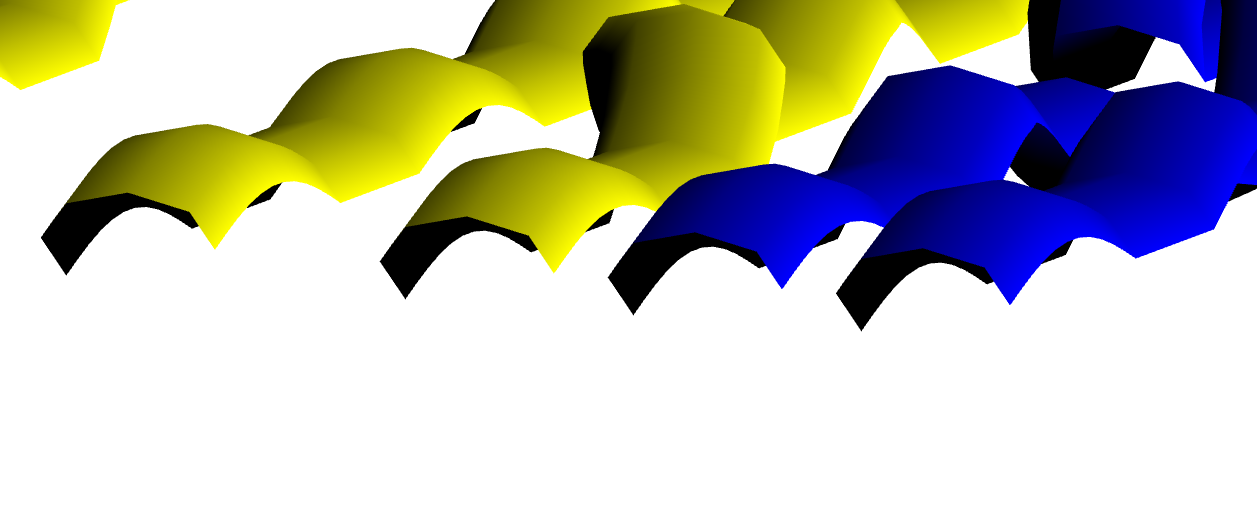
\includegraphics[width = .95\linewidth]{../cylindres.png}
            \caption{Courbes en forme de demi-cylindres}
        \end{subfigure}
        \begin{subfigure}[t]{.4\textwidth}
            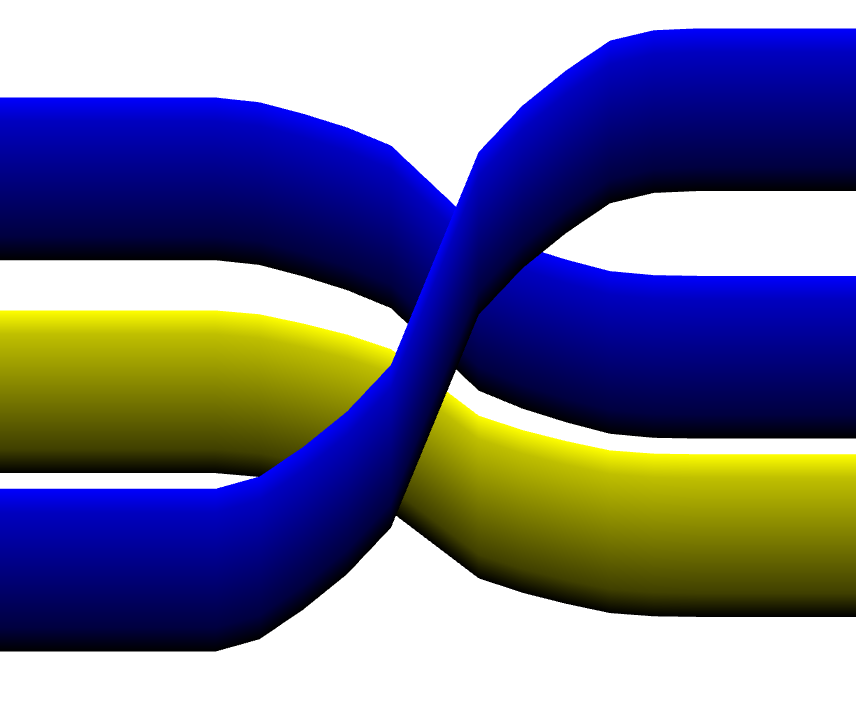
\includegraphics[width = .95\linewidth]{../courbeS2D.png}
            \caption{Courbe en S}\label{S}
        \end{subfigure}
        \caption{Création des courbes}

    \end{figure}

    Pour aller un peu plus loin, nous avons lissé les courbes pour leur donner un aspect de \textbf{S} (voir la Figure~\ref{S}).
    Pour cela, on divise en 11 intervalles la "pente" que l'on remplace par une sigmoïde.
    La fonction suivante décrit notre \textbf{S}, $f: x \mapsto \frac{1}{1 - e^{-x}}$, et on l'adapte à nos besoin en y ajoutant un facteur $a\in\mathbb{R}$ et une ordonnée à l'origine $b\in\mathbb{R}$.
    \section{Arcs de cercle}\label{sec:arcs-de-cercle}
    \begin{figure}[h!]
        \begin{subfigure}[t]{.4\textwidth}
            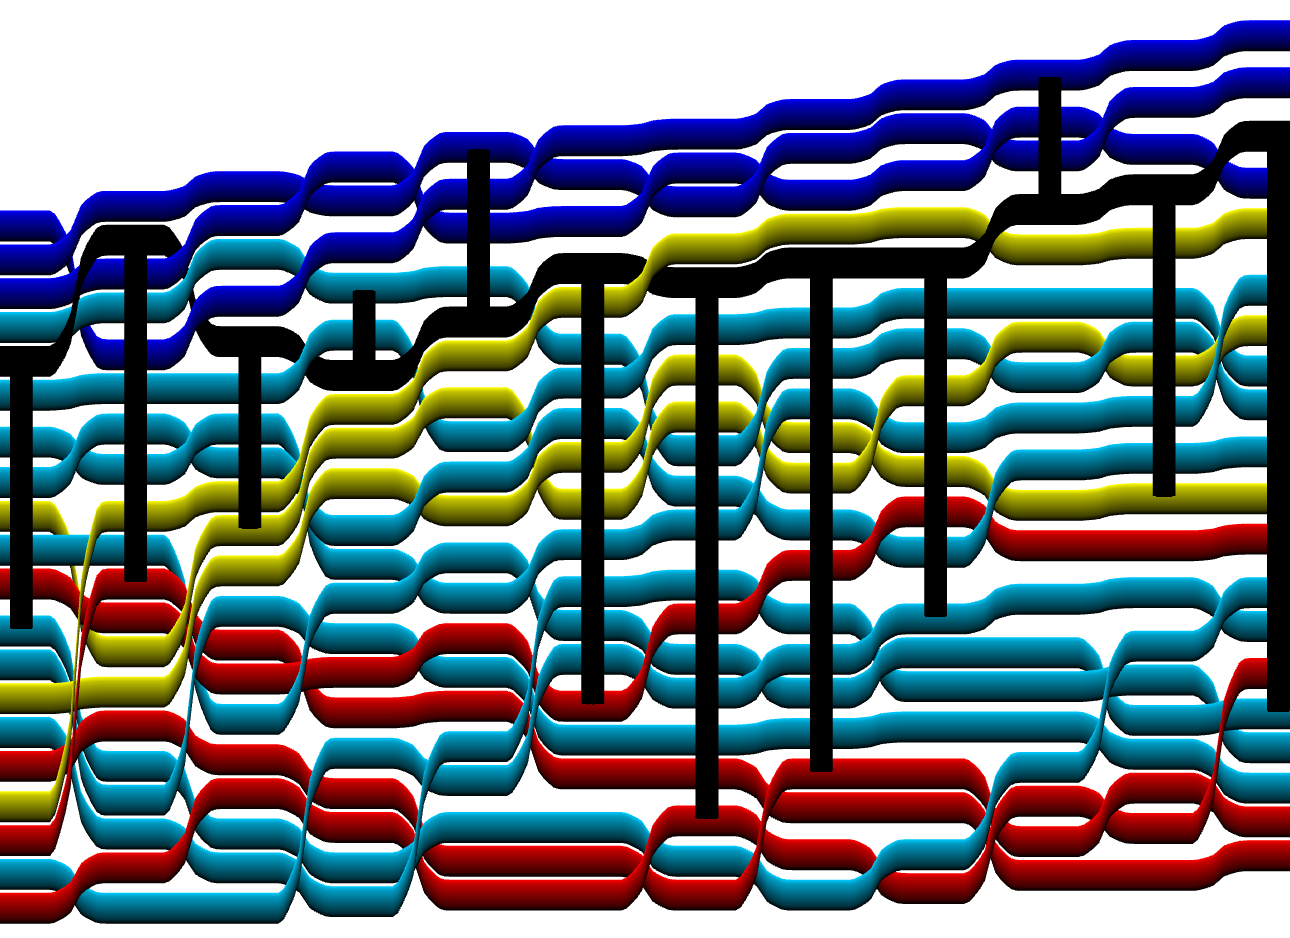
\includegraphics[width = .95\linewidth]{../arc2D.png}
            \caption{Arcs de cercle en vue 2D}
        \end{subfigure}
        \begin{subfigure}[t]{.7\textwidth}
            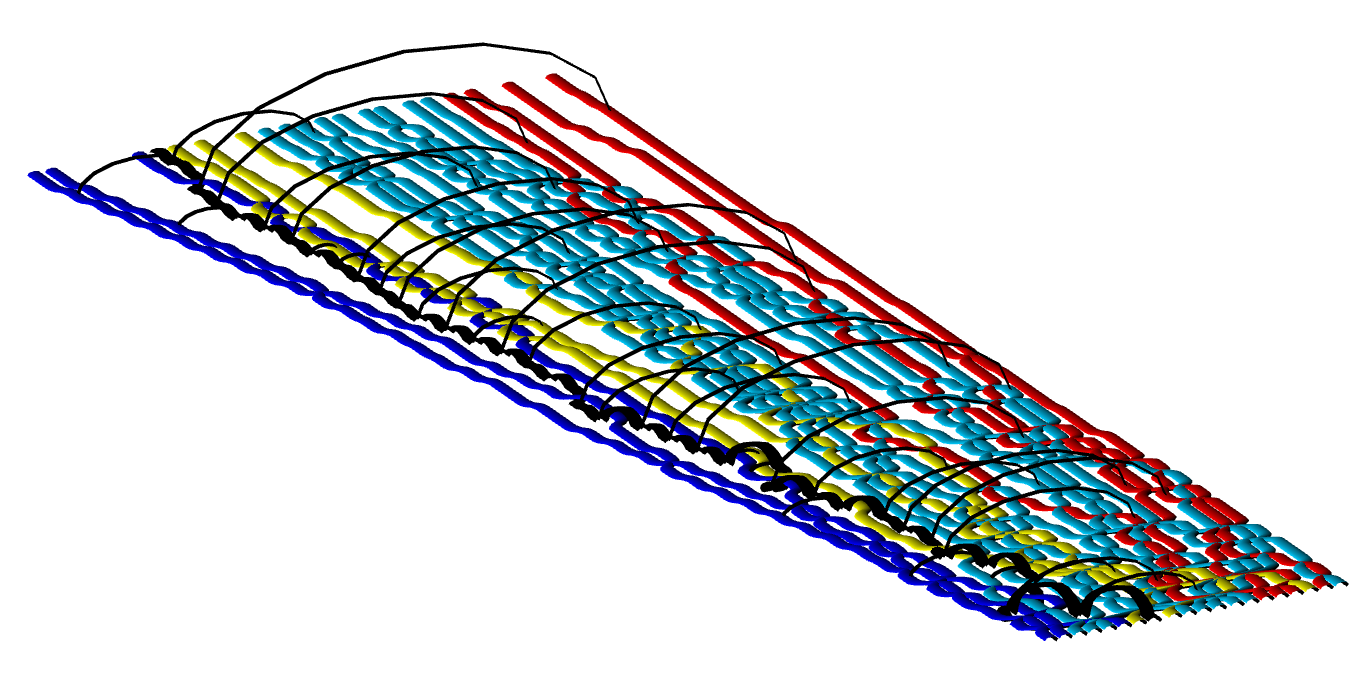
\includegraphics[width = .95\linewidth]{../arc3D.png}
            \caption{Arcs de cercle en vue 3D}
        \end{subfigure}
        \caption{Arcs de cercle}\label{arc}
    \end{figure}
    \newpage

    Pour aller encore plus loin, nous avons implémenté les arcs de cercle entre une équipe séléctionnée et ses opposants lors des matchs de football.
    Un VBO dédié a été créé et chaque arc de cercle est lui-même un cylindre complet.
    Les normales n'ont pas été utilisée donc le rayon du cylindre n'est pas toujours le même.


    \chapter{Couleur et ombrage}\label{ch:couleur-et-ombrage}
    \section{Interpolation}\label{sec:interpolation}

    \begin{figure}[h!]
        \centering
        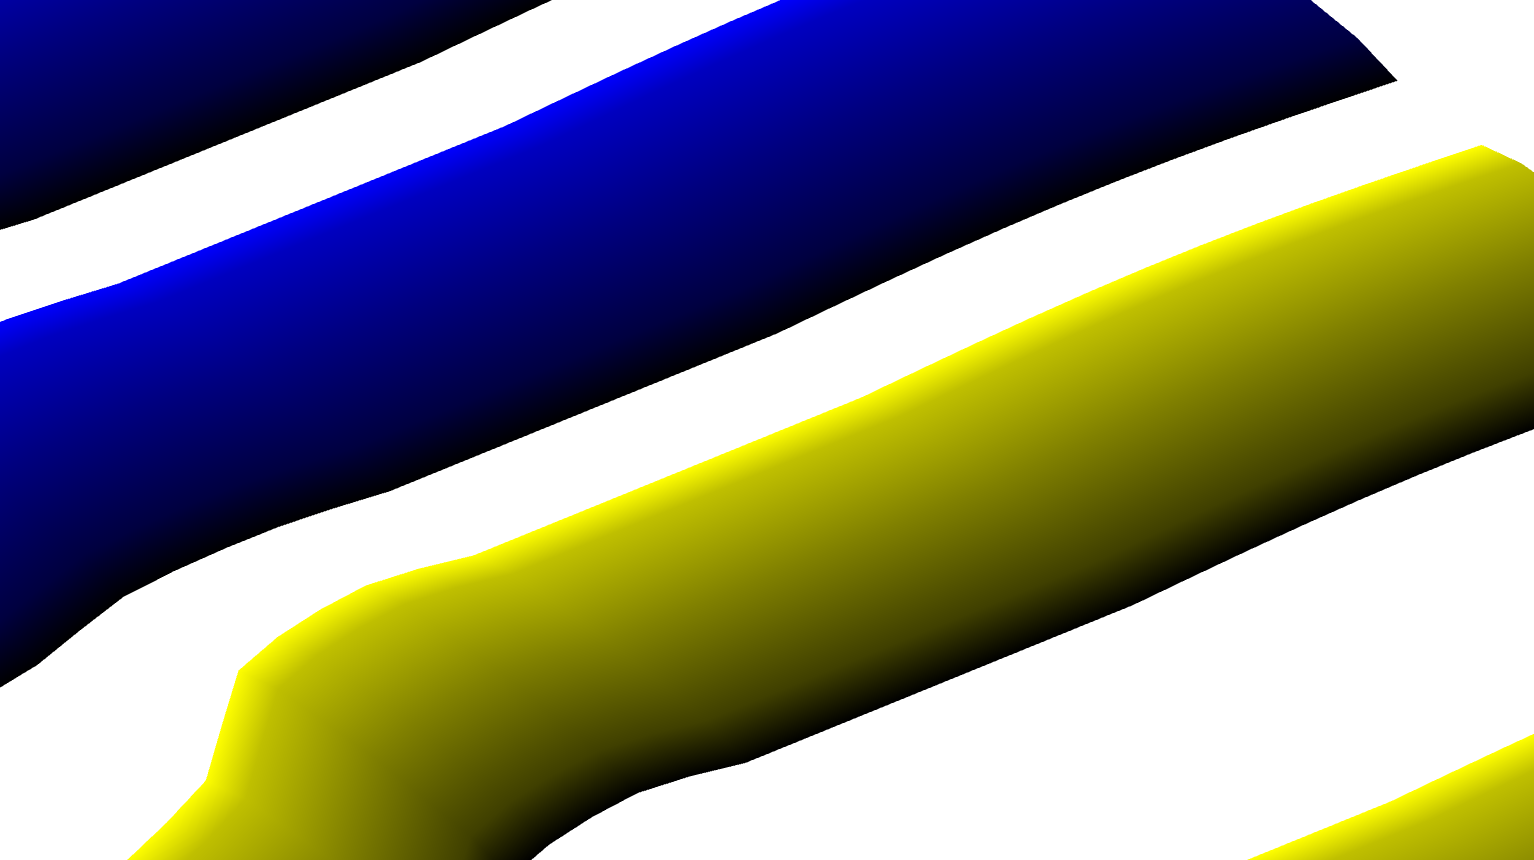
\includegraphics[width=13cm, height=6cm]{../interpolation.png}
        \caption{Interpolation des couleurs}
    \end{figure}

    Nous avons bien les courbes coloriées avec leurs couleurs respectives.
    On a interpolé les couleurs pour obtenir un dégradé clair $\to$ foncé qui donne l'aspect de l'ombre.
    \newpage

    \section{Non croisement}\label{sec:non-croisement}
    \begin{figure}[h!]
        \begin{subfigure}[t]{.5\textwidth}
            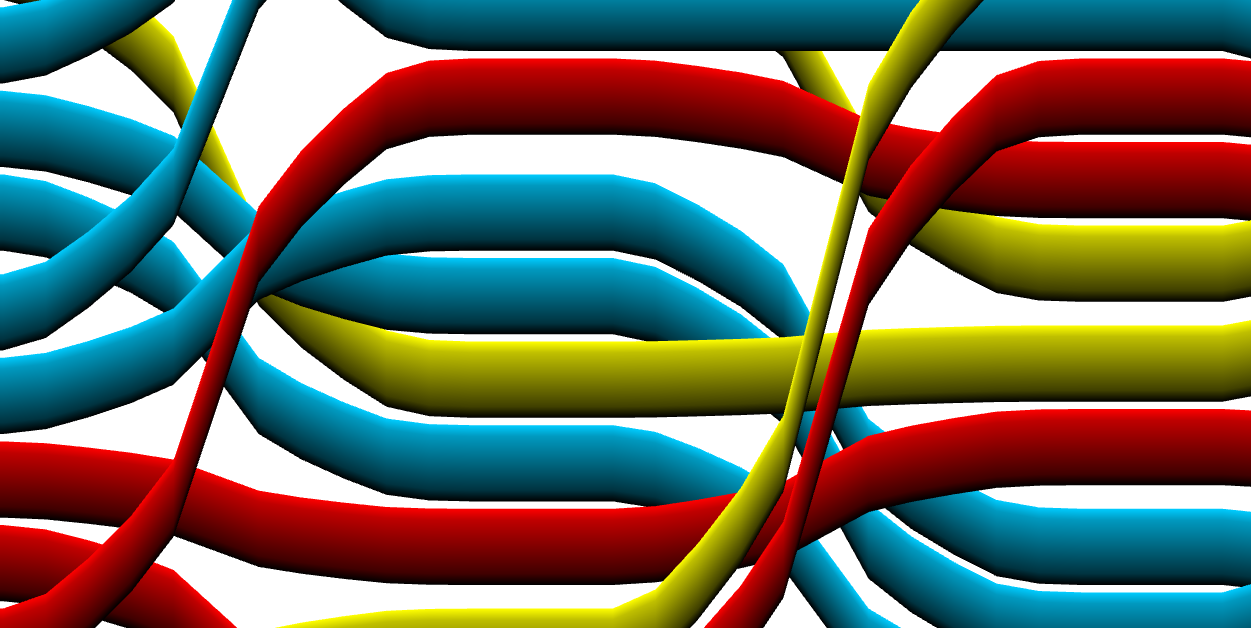
\includegraphics[width = .95\linewidth]{../auDessus2D.png}
            \caption{Vue en 2D}
        \end{subfigure}
        \begin{subfigure}[t]{.5\textwidth}
            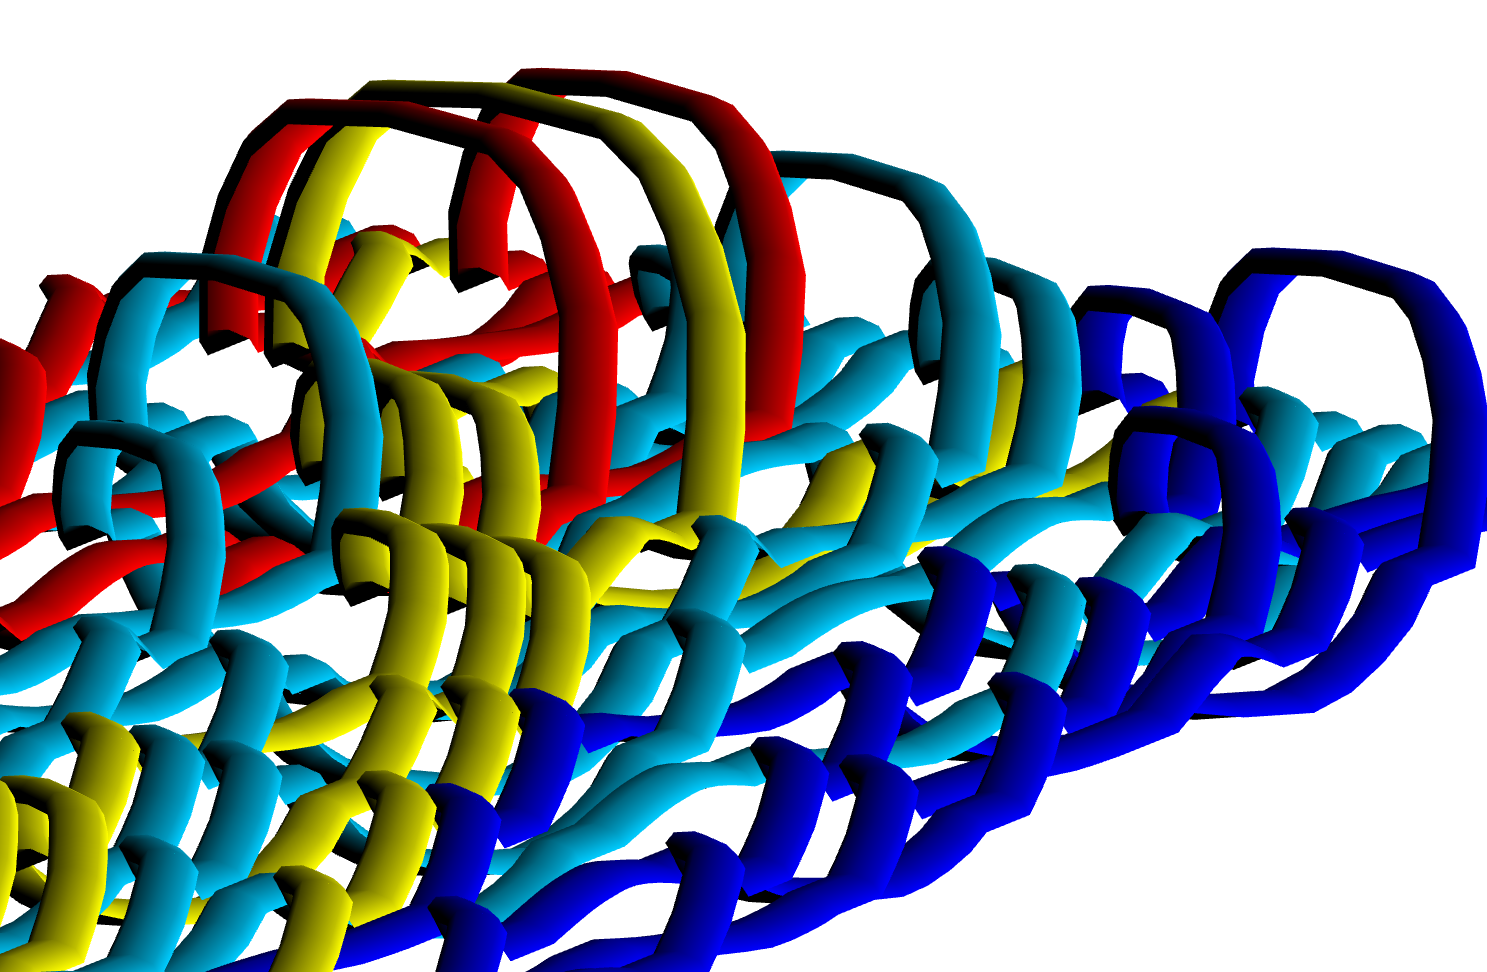
\includegraphics[width = .95\linewidth]{../auDessus3D.png}
            \caption{Vue en 3D}
        \end{subfigure}
        \begin{subfigure}[t]{\textwidth}
            \centering
            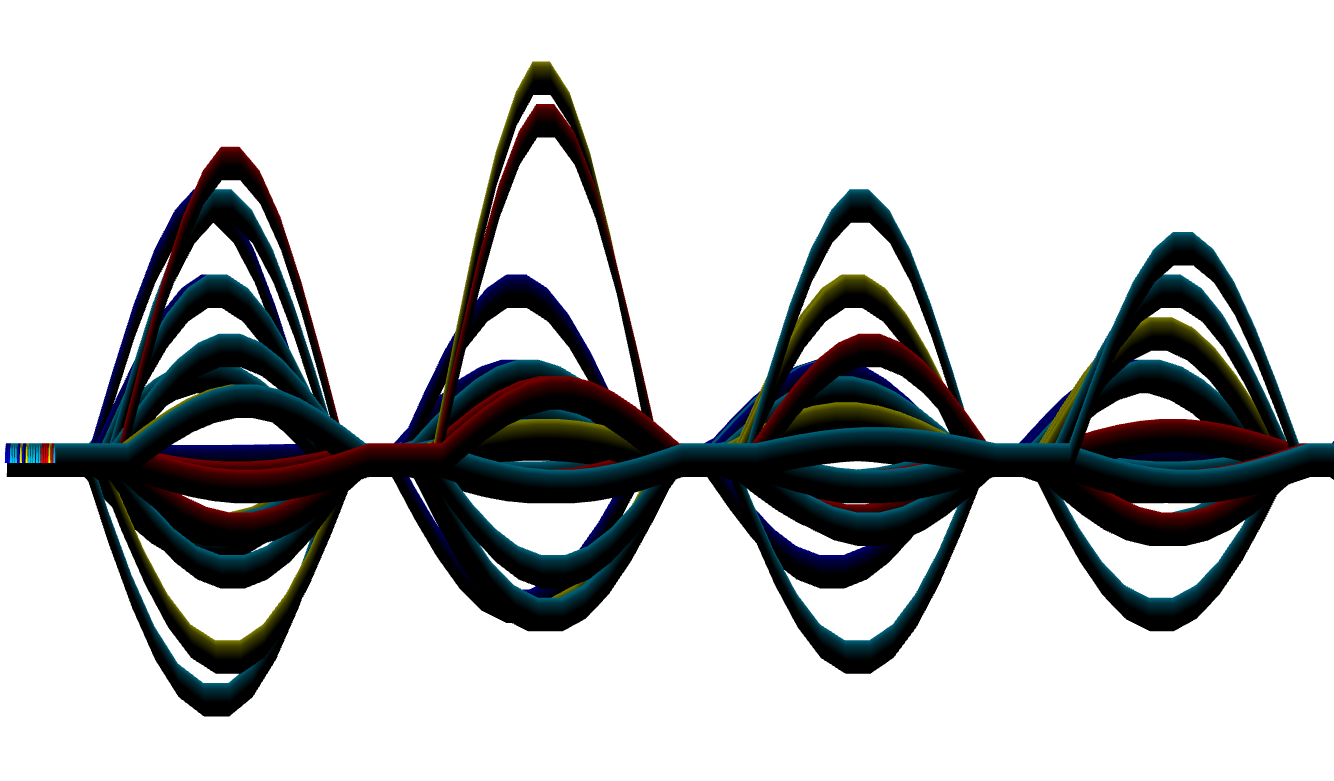
\includegraphics[width = .4\linewidth]{../auDessusCoupe.png}
            \caption{Vue en coupe}\label{sin}
        \end{subfigure}
        \caption{Les courbes ne se coupent pas}
    \end{figure}
    Pour que les courbes de se croisent pas, on a appliqué la fonction $z\mapsto \sin(z)$ sur l'axe $z$ de nos sigmoïdes, comme on peut le voir sur la Figure~\ref{sin}.
    La hauteur du sinus dépend du taux de variation de la courbe après un match.

    \chapter{Intéraction}\label{ch:intéraction}

    \section{Caméra 2D}\label{sec:caméra-2d}
    La caméra 2D est une vue du dessus de nos courbes.
    On peut déplacer la caméra perpendiculairement au plan $(x,y)$ avec Z,Q,S,D ou les flèches directionnels.
    On peut également utiliser la souris en cliquant pour déplacer la caméra.
    La molette ou les touches A,E sont utilisées pour zoomer.
    \section{Caméra 3D}\label{sec:caméra-3d}
    On peut déplacer le point où la caméra "regarde" avec le clique droit.
    On peut effectuer des rotations autour d'un axe parallèle à z avec la souris en cliquant, et avec Q,D et les flèches gauche et droite.
    On peut activer la rotation automatique avec R\@.
    On peut diminuer la hauteur de la caméra et simuler une rotations horizontale autour du point qu'on regarde avec Z et S\@.
    La molette ou les touches A,E sont utilisées pour zoomer.
    \section{Selection d'une équipe}\label{sec:selection-d'une-équipe}
    On peut selectionner une équipe avec les touches O et L (voir \ref{sec:arcs-de-cercle} pour des exemples).
    Si une équipe est selectionnée, la courbe devient noire et les arcs de cercles sont affichés.
    Si une équipe est selectionnée et que la caméra est en mode 3D, alors le non-croisement des courbes (\ref{sec:non-croisement}) n'est plus assuré pour diminuer l'encombrement.
    On peut déséléctionner les courbes avec la touche P\@.
    \subsection*{Autre}\label{subsec:autre}
    \addcontentsline{toc}{section}{Autre}
    Un système de "tic" a été implémenté pour éviter d'activer plusieurs fois une même fonctionnalité.
    La position du centre peut être choisie en mode 2D et sera la même si l'on passe en mode 3D\@.
    \begin{itemize}
        \item SPACE pour changer du mode 2D au mode 3D, et inversement
        \item + et - pour changer le rayon des arcs de cercle
        \item B et N pour changer l'étalement des sigmoïdes en $x$
    \end{itemize}


\end{document}